% Chapter 3

\chapter{Propuesta} % Main chapter title

\label{Chapter3} % For referencing the chapter elsewhere, use \ref{Chapter1} 

%----------------------------------------------------------------------------------------

\newcommand{\nmodels}{$n$ \todo{?`cuantos modelos?}}

La propuesta consta de \nmodels modelos, pensados para el análisis de texto en redes sociales como Twitter en aras de realizar un perfilado de ciber-criminales potenciales, esto por medio de \gls{nlp}, de donde se parte varias metodologías que hacen uso de tecnologías \mbox{Estado-del-Arte}.

\section{Análisis}
\todo{averiguar que se pone en esta sección}

\section{Diseño}
Como parte de la propuesta se proponen \nmodels modelos para tratar diferentes aspectos en perfilado de donde se representan los diferentes modelos en la \figureref{fig:proposal-arch}.

\begin{figure}[H]
  \centering
  \missingfigure{Hacer la arquitectura en yEd}
% 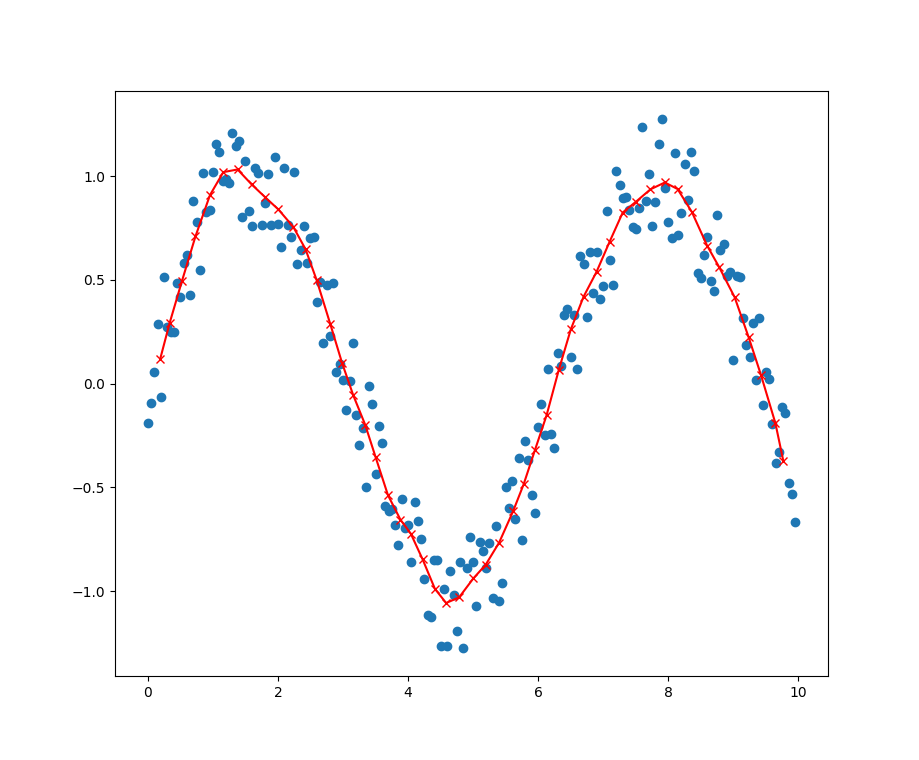
\includegraphics[scale=0.5]{Figures/som-implementation-example.png}
\decoRule
\caption[Arquitectura de propuesta]{Arquitectura de propuesta.}
\label{fig:proposal-arch}
\end{figure}

\subsection{Predicción de etiquetas de Twitter con modelos lineales}
En Twitter, las publicaciones que se realizan tienen la posibilidad de incluir menciones de temas de tendencia por el conocido \emph{hashtag}, escrito como \texttt{\#Tema}, y tiene la gran utilidad de realizar una mención explicita del tema que se quiere tratar y donde además la tarea de encontrar textos directamente relacionados con un tema son fácilmente localizables.

Así mismo, en la literatura de \gls{nlp} es muy común el uso de diferentes representaciones de palabras o conjuntos de palabras. Una representación de palabras típicas es por medio de los \gls{bow}, donde se establece un diccionario de palabras de tamaño $N$, y donde cada palabra tiene un vector que lo representa. A cada palabra se le asigna un identificador único en ese diccionario, por lo que existiría una traducción de palabra a identificador y una secuencia de palabras para poder ser recuperado por medio del índice, como se muestra en la \equationref{eq:bow-repr1} y la \equationref{eq:bow-repr2}.
\begin{equation} \label{eq:bow-repr1}
  \text{word2idx} = \Big\{(\text{word}_i, i) : \forall i \in [1, \ldots, N] \Big\}
\end{equation}

\begin{equation} \label{eq:bow-repr2}
  \text{idx2word} = \Big[\text{word}_i\Big], \forall i \in [1, \ldots, N]
\end{equation}

Otra representación común en \gls{nlp} es la de \gls{tfidf}, que se divide en dos partes, expresadas en las \equationref{eq:tf-repr}, la \equationref{eq:idf-repr} y la composición de ambas en la \equationref{eq:tfidf-repr}, $D$ es el corpus de palabras. Este consiste en penalizar palabras que ocurren mucho en un documento pero no mucho en el corpus o bien de penalizar la palabras que se repiten poco en un documento pero se repiten mucho en el corpus, por lo que un punto medio entre ambos es recompensado.

\begin{equation} \label{eq:tf-repr}
  \text{tf}(t,d) = \text{Frecuencia del termino (o n--grama) } t \text{ en el documento } d
\end{equation}

Existen diferentes variaciones para realizar representar el conteo de términos \textbf{tf} de forma normalizada, como se representa en el \tableref{table:tf}.

\begin{table}[h!]
\centering
\begin{tabular}{|l|l|} \hline
  \textbf{Esquema}          & \textbf{Peso de tf} \\ \hline
  Binario                   & $0, 1$ \\ \hline
  Conteo directo            & $f_{t, d}$ \\ \hline
  Frecuencia de términos    & $f_{t, d} / \sum_{t' \in d}f_{t', d}$ \\ \hline
  Normalización logarítmica & $1 + \text{log}(f_{f, d})$ \\ \hline
\end{tabular}
\caption{Variaciones de \textbf{tf}}
\label{table:tf}
\end{table}

\begin{equation} \label{eq:idf-repr}
  \text{idf}(t, D) = \text{log}\Bigg( \frac{N}{|\{d \in D : t \in d\}|} \Bigg) ; N = |D|
\end{equation}

\begin{equation} \label{eq:tfidf-repr}
  \text{tfidf}(t, d, D) = \text{tf}(t, d) \cdot \text{idf}(t, D)
\end{equation}

\subsection{Reconocimiento de entidades nombradas con redes \glsentrylong{lstm}}
\todo{Pendiente} Bla

\subsection{Búsqueda de tweets relacionados con \emph{embeddings} de StarSpace}
\todo{Pendiente} Bla


\section{Resultados}
\lipsum
